\documentclass[conference]{IEEEtran}
\usepackage{blindtext, graphicx}
\usepackage{cite} 
\usepackage{csquotes}
\usepackage[hidelinks]{hyperref}
\usepackage{url}
\usepackage{pgfplots}
\usepackage{booktabs}

\hyphenation{op-tical net-works semi-conduc-tor}

\begin{document}
\title{Using Natural Language Processing in a job interview to judge employer's required skills from employees}

% The sequence of authors in a paper has meaning. The first to be listed is known as the First Author, who is usually the student and/or the person doing the bulk of the work. The next in line, provided that there are two persons, is called the corresponding author, also known as the technical mentor/supervisor. Any person who is consulting, correcting or verifying such as a second reader or senior person within the Faculty/Institute is listed after the previous authors.

\author{\IEEEauthorblockN{Kyle Vella}
\IEEEauthorblockA{Institute of Information \& Communication Technology\\
Malta College or Arts, Science \& Technology\\
Corradino Hill\\
Paola PLA 9032\\
\{kyle.vella.g52651\}@mcast.edu.mt}}

\maketitle

\begin{abstract}
Traditional recruitment process comes with high operation costs and human bias. Due to corporations shift towards Industry 4.0, use of automated machines scoring has increased due to capabilites of interpreting qualitative data. This research develops and validates an interview prototype containing BART-MNLI Zero Shot Classifier installation to score open responses bsaed on Big Five personality traits. Pearson Correlation was utilized to validate by comparing AI scores and human recruit scores. Results found a moderate positve relation (0.5286) and a 99 percent decrease in processing time compared to manual scoring. However, error analysis reveals lack of understanding in terms regarding industry-specifc terms or technical acronyms. Findings suggest tuning on large language model's datasets to improve scoring accuracy across industry recruitment sectors.  
\end{abstract}

\begin{IEEEkeywords}
%3 to 5 words/phrases about the key aspects of your research, theme, technology, technique
Personality, traits, zero shot classifer, scoring
\end{IEEEkeywords}

\IEEEpeerreviewmaketitle

\section{Introduction}
\label{sec:Int}
\par The introduction is intended to give a more detailed overview of the research from the abstract. Document the \textbf{theme}, the \textbf{aim} and \textbf{motivation}. By motivation we mean the justification to why this project/research is relevant/needed for the current year/period and for your specific area of studies. You can consider also including your \textbf{hypothesis} and \textbf{research questions} in this section. Conclude this section with an overview of what to expect in the next sections. It is good practice to cross-reference your own paper using the ref command for the matching section label, such as in Section~\ref{sec:Lit} a review of current research is found.
\par Due to shift towards “Industry 4.0”, companies were forced to seek automated solutions for hiring. With rise of Transformer-based models using Natural Language Inference (NLI), it allows machines to understand the intent behind a candidate's story. The aim of this research was to develop and validate an interview prototype utilizing Zero-Shot NLP to provide real-time scoring of candidates personality traits. Traditional interview are prone to bias and expenses to run an interview. With use of BART-MNLI, it prevents lacking qualitative depth of conversation while employing automated scoring based on required labels from open-ended answers. 
\section{Literature Review}
\label{sec:Lit}
\par Give a \textbf{brief} overview of the theme, history and facts. You should use the present tense since what you are documenting is current knowledge. Do not dedicate a lot to historical facts about the subject matter, but limit to a paragraph. Make sure you quantify by quoting statistics where relevant. Following is an example for a research in \enquote{Automatic cyber-bullying detection}: \textit{With the popularity of social media, predominantly amongst the adolescent and young adult generations, there appears to be a correlation between the increase in suicide rates and social networking adoption~\cite{miron2019suicide}, with suicide attempts increasing by 10\% amongst adolescents and by 5.6\% amongst young adults for the period 2013-2017.} 

\par Due to shift towards “Industry 4.0”, companies were forced to seek automated solutions for hiring. With rise of Transformer-based models using Natural Language Inference (NLI), it allows machines to understand the intent behind a candidate’s story. Candidate's personality scoring relied on interviews, although unstrcuted interviews are known to be 20 to 30 percent predictable due to human error and human bias \cite{pansare2022pppkosam}. Since Natural Language processing has evolved, Large Language Models being the norm in every industry enables machines to score human personality traits from open ended response accurately. Literature review analyses use, performance, and accuracy of large language models in personality assesment 

\par A. Pansare, P. Panwar, and P. Kosamkar \cite{pansare2022pppkosam} conducted a comparative study on natural language processing systems based on predicting personalities. Researchers used an MBTI dataset containing 8670 rows (personality set and fifty recent tweets) and two columns where it represents mostly all personality types. All tweets collected and questionnaire was used to judge the participants personality. The system, developed by researchers, consists of Logistic Regression, Random Forest Algorithm, Support Vector Machines, and XGBoost. Results found that the system scored high accuracy scores with thinking/feeling attribute being the highest, but lowest being perceiving vs judging. 

\par S. R. Karra, S. T Nguyen, and T. Tulabandhula \cite{Karra:2022} conducted a comparative study from large language models on judging participants personality based on answers with use of Big Five Factors (Extraversion, Neuroticism, Agreeableness, Conscientiousness, Openness). Researchers used labels (each label has two ends such as from extroversion to introversion) on zero shot classifiers (ZSC), which are large language models, to judge the participants answers. Researchers used pre-processed datasets, from BookCorpus and Wikipedia, containing both sentences and small paragraphs for the ZSC to judge on. 

\par S. Sikström, I. Valavičiūtė, and P. Kajonius \cite{s2025sikstrom} analysed the validity of NLP judging personality based on word-based responses. 663 participants were recruited from United States of America, United Kingdom, and other countries with use of Prolific.io which is an online recruitment tool to collect data. The session consists of two phases. Phase 1 was where participants wrote a description about own or someone else’s specific personality trait with use of keywords and no mention of personality trait. Phase 2 was where other participants read participant’s written description. IPIP-NEO-30, derived from International Personality Item Pool, was used to measure, measured by participants, five personality factors, extraversion, openness, agreeableness, conscientiousness, and neuroticism. Demographic information such as age, gender, birth of country, education and confidence level were collected with use of questionnaires. The user-made descriptions, written in Microsoft Word, were analysed with use of GPT-4 and BERT based on the big five personality traits. Results found higher prediction accuracy than the rating scale, higher reliability, and better observation than self-report. 

\par J. Kurek et al. \cite{j2024kurek} conducted comparative study on zero shot classifier as a recruitment tool. Dataset contained unique job candidates, unique jobs, and matches between jobs and candidates totalling up to 3169 records. Only English documents were used only used due to researchers focus on English documents only. Models such as all-MiniLM-L2-v2 and LaBSe were selected by the researchers due to “models’ ability to produce embedding vector representations that accurately capture semantic meanings”. Results found high accuracy scores, importance of selecting the appropriate model as a recruitment tool, high performance, and recommended modifications on pre-trained models. 

\par L. Hu et al. \cite{lhu2024llm} made use of large language model (LLM) to analyse personality based on user’s input. Researchers collected user’s posts (from Kaggle and Pandora) which was used on LLM, GPT 3.5 Turbo, to analyse from three perspectives (semantic, sentiment, and linguistic perspective). Prompts were made to LLM to generate explanation on each MBTI trait and calculate similarity between the user and the label description with use of soft labels. Results found that the model, constructed by the researchers, outperformed all traditional methods that detect personalities, performance impact from focus on linguistic over semantic, and struggles to generate explanations with use of LLMs rather than specific small models. Limitations include limited dataset, and input length.

\par All sources touched on use of LLMs and NLPs in the context of job recruitment. Referenced studies made use of GPT-4, BERT, and BART as zero shot classifiers, and Logistic Regression, Random Forest, and XGBoost to predict personality traits from social media datasets. Pansare et al. \cite{pansare2022pppkosam} made use of specific models such as XGBoost, and Random Forest resulted in high accuracy but required large and pre-labelled datasets. On the other hand, Karra et al. \cite{Karra:2022} and Kurek et al. \cite{j2024kurek} employed Zero-shot classifiers showed that personality scoring was able to  be executed without specific training, supported by Sikstrom et al. \cite{s2025sikstrom} who found that GPT-4 offered high reliability than self-report scales. Although LLMs outperform traditional methods, LLMs often struggle to generate explanation based on traits compared to smaller specific models. In addition, Kurek et al. \cite{j2024kurek} identified a linguistic gap due to limiting found documents to only English, as well as Hu et al. finding performance gaps when focus shifts to linguistic perspectives over semantics. Limitations found in this literature review represent a knowledge gap that the research gap needed to be addressed in this research by using BART-MNLI to evaluate and score open-ended candidate stories. 

\par Finally, sources reviewed in the literature review were peer-reviewed and contained in-depth analysis, differed from non-academic sources that lacks evidential findings due to lack of analysis and use of biased sources. By putting focus on academic work, this literature review identified technical gaps such as linguistic constraints and bias driven by pretrained data. However, non-academic material would only provide benefits of use of AI, but do not provide any findings based on limitations found in academic work. 

\begin{table}[htbp]
\centering
\caption{Comparative Analysis of Literature: Data, Algorithms, and Metrics}
\label{tab:LitComparison}
\resizebox{\columnwidth}{!}{%
\begin{tabular}{|l|l|l|l|}
\hline
\textbf{Source} & \textbf{Data Set Type} & \textbf{Algorithm/Model} & \textbf{Primary Metric} \\ \hline
Pansare [1] & Social Media (MBTI) & XGBoost / Random Forest & Accuracy \\ \hline
Karra [2] & Wikipedia/Corpus & Zero-Shot (LLM) & Semantic Mapping \\ \hline
Sikström [3] & Prolific.io Narratives & GPT-4 / BERT & Pearson Correlation \\ \hline
Kurek [4] & Job-Matching Data & all-MiniLM / LaBSE & Matching Score \\ \hline
Hu [5] & Kaggle/Pandora Posts & GPT-3.5 Turbo & Soft Labels \\ \hline
\end{tabular}
}
\end{table}

\begin{figure}[ht]
    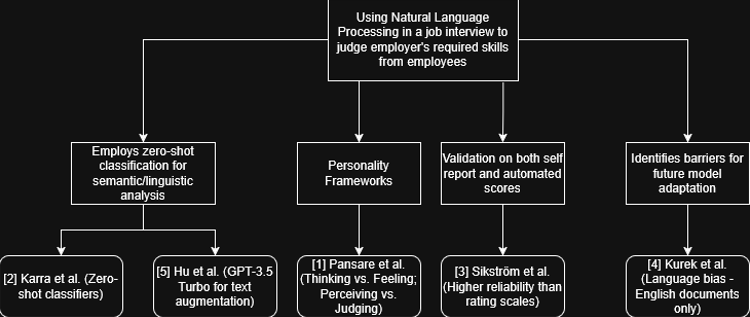
\includegraphics[scale=0.5]{includes/litmap.png}
    \centering
    \caption{Literature Map}
    \label{fig:Map}
\end{figure}
\section{Research Methodology}
\label{sec:Res}
\par This section is one of the most important parts of your research and it is the one that will receive most criticism. The reason is that here you document how you conducted your research. Since you are reading a B.Sc. degree you are expected to follow a scientific method, thus in this section you are expected to document: \textbf{the problem}; \textbf{hypothesis}; \textbf{aim \& objectives}; \textbf{research questions}; and \textbf{research pipeline}. Let's go through each.

\par Traditional interview are prone to bias and expenses to run an interview. With use of BART-MNLI, it prevents lacking qualitative depth of conversation while employing automated scoring based on required labels from open-ended answers. The research hyptohesized that \textit{there is a significant positive correlation between the semantic scores generated by the BART-MNLI model and the evaluation scores provided by expert human recruiters for the same set of open-ended responses.}

\par The primary aim of this reserach was to develop and make use of a simple python app that utilized Zero-Shot Natrual Language Processing to display real-time assesment of candidate personality traits based on open-ended responses.  Our research objectives were:
\begin{enumerate}
    \item Collect and simulate data set of open ended job interview responses related to specified employer skills 
    \item Implement BART-MNLI to generate a score for each user response
    \item Conduct correlation analysis between AI scores and human scores
    \item Measure and compare time taken to process automated scoring against time taken by human recruiters to evaluate users answers
    \item Conduct error analysis on instances with low correlation to detect linguistic issues or terms where ZSC fail to score.
\end{enumerate}

\par The research aimed to answer the following research questions:
\begin{enumerate}
    \item To what extent does the BART-MNLI zero-shot classification model correlate with expert human recruiter evaluations when scoring specific employer-required skills in open-ended interview responses?
    \item Does the use of automated NLI-based scoring significantly reduce the time required for the initial candidate screening phase compared to traditional human-led qualitative analysis?
    \item What are the primary linguistic limitations of the BART-MNLI model when interpreting nuanced or industry-specific terminology in candidate "stories"?
\end{enumerate}

\par Finally, you need a plan on how you intend to answer the research questions which will help you prove/disprove the hypothesis. Different research areas would require specific pipelines, yet a generic one is shown in Fig~\ref{fig:Pipeline}. After presenting an illustration of your pipeline it is recommended to documenting what has been done at every stage. Remember you should use past tense in this section since you are document what you have already done, since this paper will be published at the end of your research.

\begin{figure}[ht]
    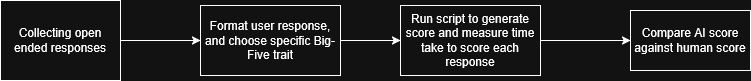
\includegraphics[scale=0.25]{includes/pipeline.png}
    \centering
    \caption{Research Pipeline}
    \label{fig:Pipeline}
\end{figure}
\section{Findings \& Discussion of Results}
\label{sec:Fin}

\subsection{AI Score vs. Recruiter Score Correlation}
\par After responses from 4 participants, both AI and human reviewer scores calculate a pearson correlation of 0.5286 resulting in a moderate positive relationship as show in figure \ref{fig:correlation_plot}. The prototype was proven to be used as a supportive rather than replacing human reviewers. 

\begin{figure}[htbp]
    \centering
    \footnotesize \small
    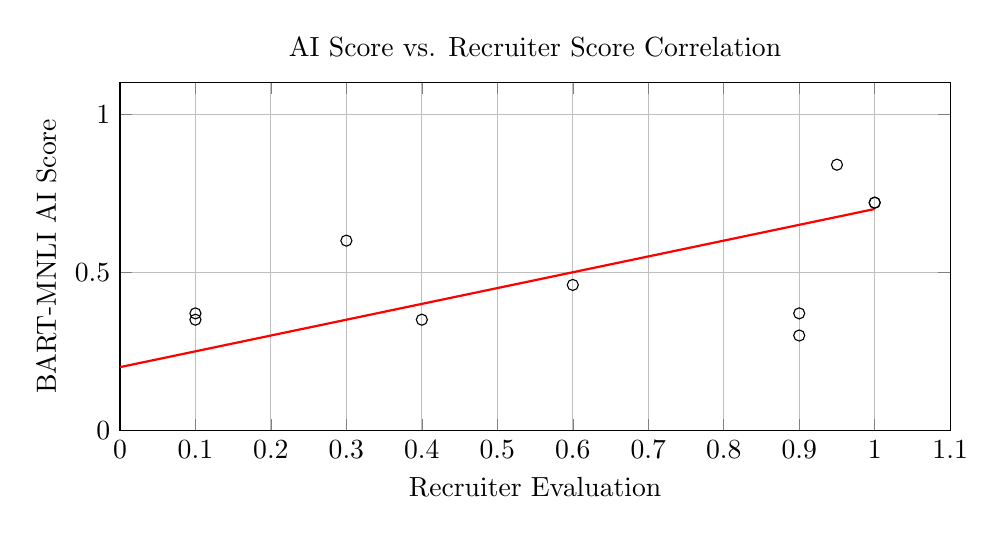
\begin{tikzpicture}
    \begin{axis}[
        width= \columnwidth,
        height= 6cm,
        title={AI Score vs. Recruiter Score Correlation},
        xlabel={Recruiter Evaluation},
        ylabel={BART-MNLI AI Score},
        xmin=0, xmax=1.1,
        ymin=0, ymax=1.1,
        grid=major,
        scatter/classes={
            a={mark=o,draw=black}}
    ]
    \addplot[
        scatter,
        only marks,
        mark size=2pt,
        scatter src=explicit symbolic
    ] table [meta=label] {
        x y label
        0.90 0.30 a
        1.00 0.72 a
        1.00 0.72 a
        0.95 0.84 a
        0.90 0.37 a
        0.40 0.35 a
        0.60 0.46 a
        0.10 0.37 a
        0.30 0.60 a
        0.10 0.35 a
    };
    % Regression Line (Approximate for r=0.52)
    \addplot [red, thick, domain=0:1] {0.5*x + 0.2};
    \end{axis}
    \end{tikzpicture}
    \caption{Scatter plot illustrating the moderate positive correlation ($r = 0.5286$) between automated and manual scoring.}
    \label{fig:correlation_plot}
\end{figure}

\par However, ZSC struggled to identify key terms found in user's open ended responses. For instance, the term 'SLA' was scored higher by the human recruiter than AI. BART-MNLI was trained on general sources such as wikipedia which possesses misunderstanding the industry context.  

\par The results align with Sikström et. al \cite{s2025sikstrom} since the source stated that Natural Language Processing is sensitive to specific word choice such as technological terms. This confirmed Sikström's theory where artifiical intelligence scoring significantly change if some words are subtle. 

\par In the session, model's confidence score dropped if the user's open response is shorter than 20 words resulting in a minimum character count. 

\begin{table}[htbp]
    \centering
    \caption{Comparative Analysis of AI vs. Recruiter Scoring for Selected Responses}
    \label{tab:Comparison}
    \resizebox{\columnwidth}{!}{% % This scales the table to fit the column
    \begin{tabular}{llp{4cm}cc} 
        \toprule
        \textbf{ID} & \textbf{Trait} & \textbf{Candidate Response} & \textbf{AI} & \textbf{Human} \\ 
        \midrule
        0 & Cons. & I managed three simultaneous projects by using a Gantt chart... & 0.72 & 1.00 \\
        \midrule
        1 & Open. & I noticed our traditional filing system was inefficient... & 0.30 & 0.90 \\
        \midrule
        2 & Extra. & I hate talking to people I don't know. I'd much rather sit in the back... & 0.30 & 0.90 \\
        \midrule
        3 & Agree. & I don't care about making friends at work. If I think an idea is stupid, I'll say it... & 0.30 & 0.90 \\
        \midrule
        4 & Neuro. & When confronted with technical debt, I focus on root-cause analysis without escalating... & 0.30 & 0.90 \\
        \bottomrule
    \end{tabular}%
    }
\end{table}

\begin{table}[htbp]
    \centering
    \caption{Operational Efficiency Comparison: AI vs. Manual Evaluation}
    \footnotesize \small
    \resizebox{\columnwidth}{!}{
    \label{tab:Efficiency}
    \begin{tabular}{|l|c|c|}
        \hline
        \textbf{Metric} & \textbf{BART-MNLI Prototype} & \textbf{Human Recruiter} \\ \hline
        Total Evaluations & 20 & 20 \\ \hline
        Avg. Time per Response & 0.35 seconds & $\sim$60.0 seconds \\ \hline
        Total Process Time & 7.04 seconds & $\sim$20 minutes \\ \hline
        \textbf{Time Reduction} & \textbf{99.4\%} & - \\ \hline
    \end{tabular}
    }
\end{table}
\section{Conclusion}
\label{sec:Con}
\par Results found a moderate positive correlation of 0.5286 which is evidenced that AI can be used in a personality assesment. However, ZSC is shown that is suitably used as a support tool rather than a complete human recruiter replacement. Reduction on time when scoring open ended responses based on a specific Big-Five trait is massive. AI scoring was executed under a second when evaluating user's open ended response, while a human recruiter took 1-2 minutes to evaluate and score. Despite the Pearson Correlation score, it was also found AI's inability to identify linguistic and industry-speicifc terms which influenced AI's scoring. For instance, AI failed to recognise terms such as "SLA" and "CRM" in one of the user's repsonse. 

\par A primary limitation identified was small sample size which consisted of 4 users. Due to the sample size, this might have changed the validation of the prototype's use in the persoanlity assesment in the context of job recruitment. As previously stated, ZSC lacks understading in industrial specifcs due to model's general training sources. 1 human recruiter resulted in possible human bias which impacted human recruiter's scoring. In addition. BART-MNLI was only comapred in context of AI scoring which negatively impacts validation of AI's role in personality assement. 

\par Models should be fine tuned in order to improve identifying speicifc industrial terms such as HR-specific datasets. Alternatively, industry-specifc models should be used for personality assesment to combat techincal jargon. Finally, sample size should be increased by inviting more participants or make use of datasets that contains user repsonses used for personality assesment.

\appendices
\input{includes/07-Supporting}
\input{includes/08-Acknowledgements}

\bibliographystyle{IEEEtran}
\bibliography{sources.bib}

\end{document}


